In the case of focusing at low f-numbers (tight-focusing), the conventional solid state optics are inappropriate. Nevertheless, many of the drawbacks mentioned above might be overcome by using a plasma-based focusing optic. As already mentioned in the chapter 2, when the laser pulse with intensity higher than $ 10^{16} \ \mathrm{W/cm}^{2} $ hits a solid target, a thin dense plasma layer is immediately formed on its surface. Under certain conditions, the plasma becomes dense enough and the reflectivity of otherwise non-reflecting target strongly increases. The incident laser light is reflected at the critical plasma density, thus the dense plasma acts as a mirror. For this reason, such optical components are called plasma mirrors.

Plasma mirrors are able to operate under much higher energy density than the conventional solid state optics, therefore the diameter of the optics aperture can be more than one order of magnitude smaller. Consequently, plasma mirrors can be mass-produced at much lower cost, which is crucial since they are single-use and therefore have to be replaced after each shot. In addition, the concerns about damage from target debris are naturally eliminated.

To induce focusing, the surface of plasma mirror has to be curved similarly as in the case of conventional optics. However, since the distance between the mirror and the interaction region can be very small, the corresponding f-number is also small, thus enabling to focus an incident laser beam theoretically to a spot size smaller than the laser wavelength. In addition, plasma mirrors are attractive also due to their ability to improve the temporal and spatial contrast ratio of the laser pulse, which is crucial for many applications of the laser-matter interaction.

\floatsetup[figure]{style=plain, subcapbesideposition=top}
\begin{figure}[h!]
	\centering
	\sidesubfloat[]{{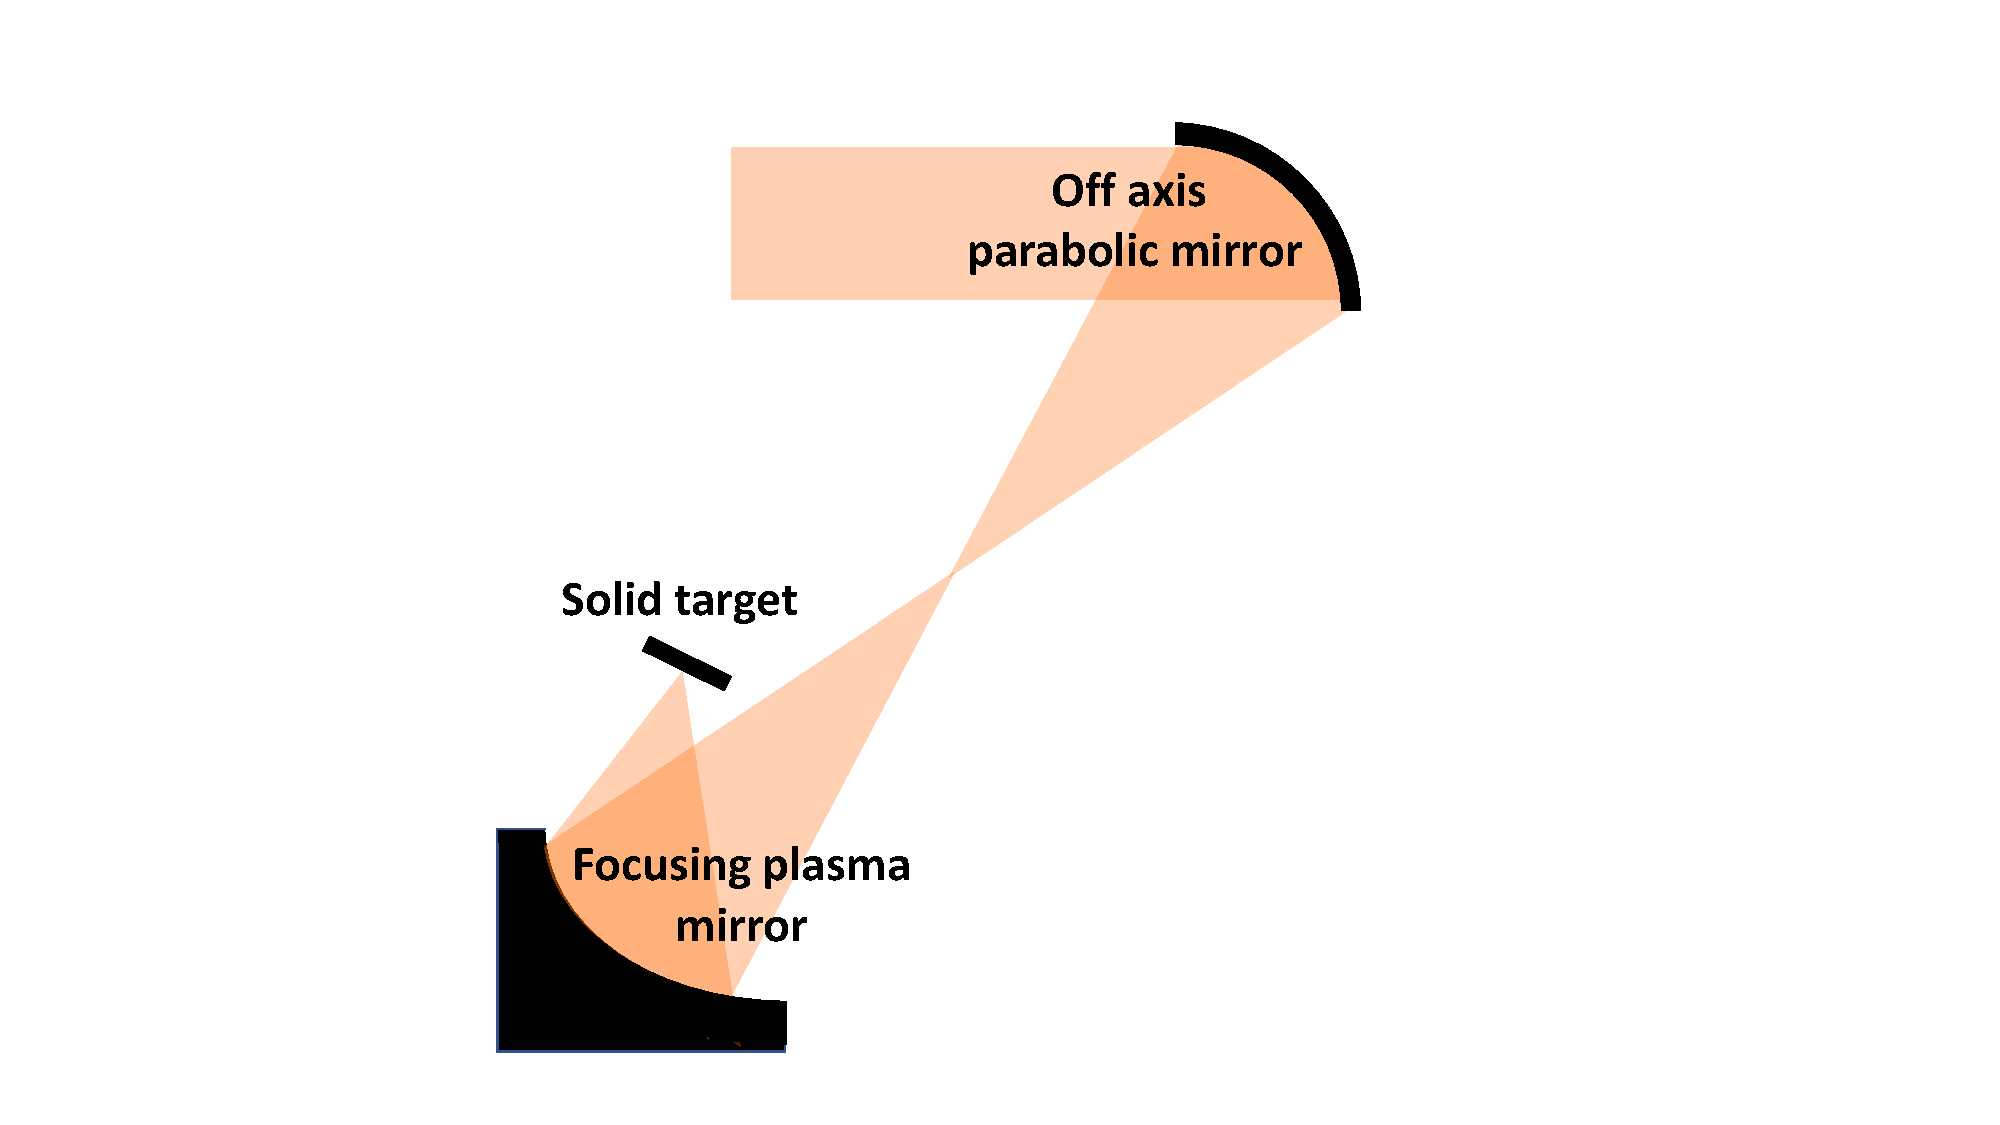
\includegraphics[width=0.35\linewidth]{./img/exp/diagram.pdf}}}
	\hspace{5mm}
	\sidesubfloat[]{{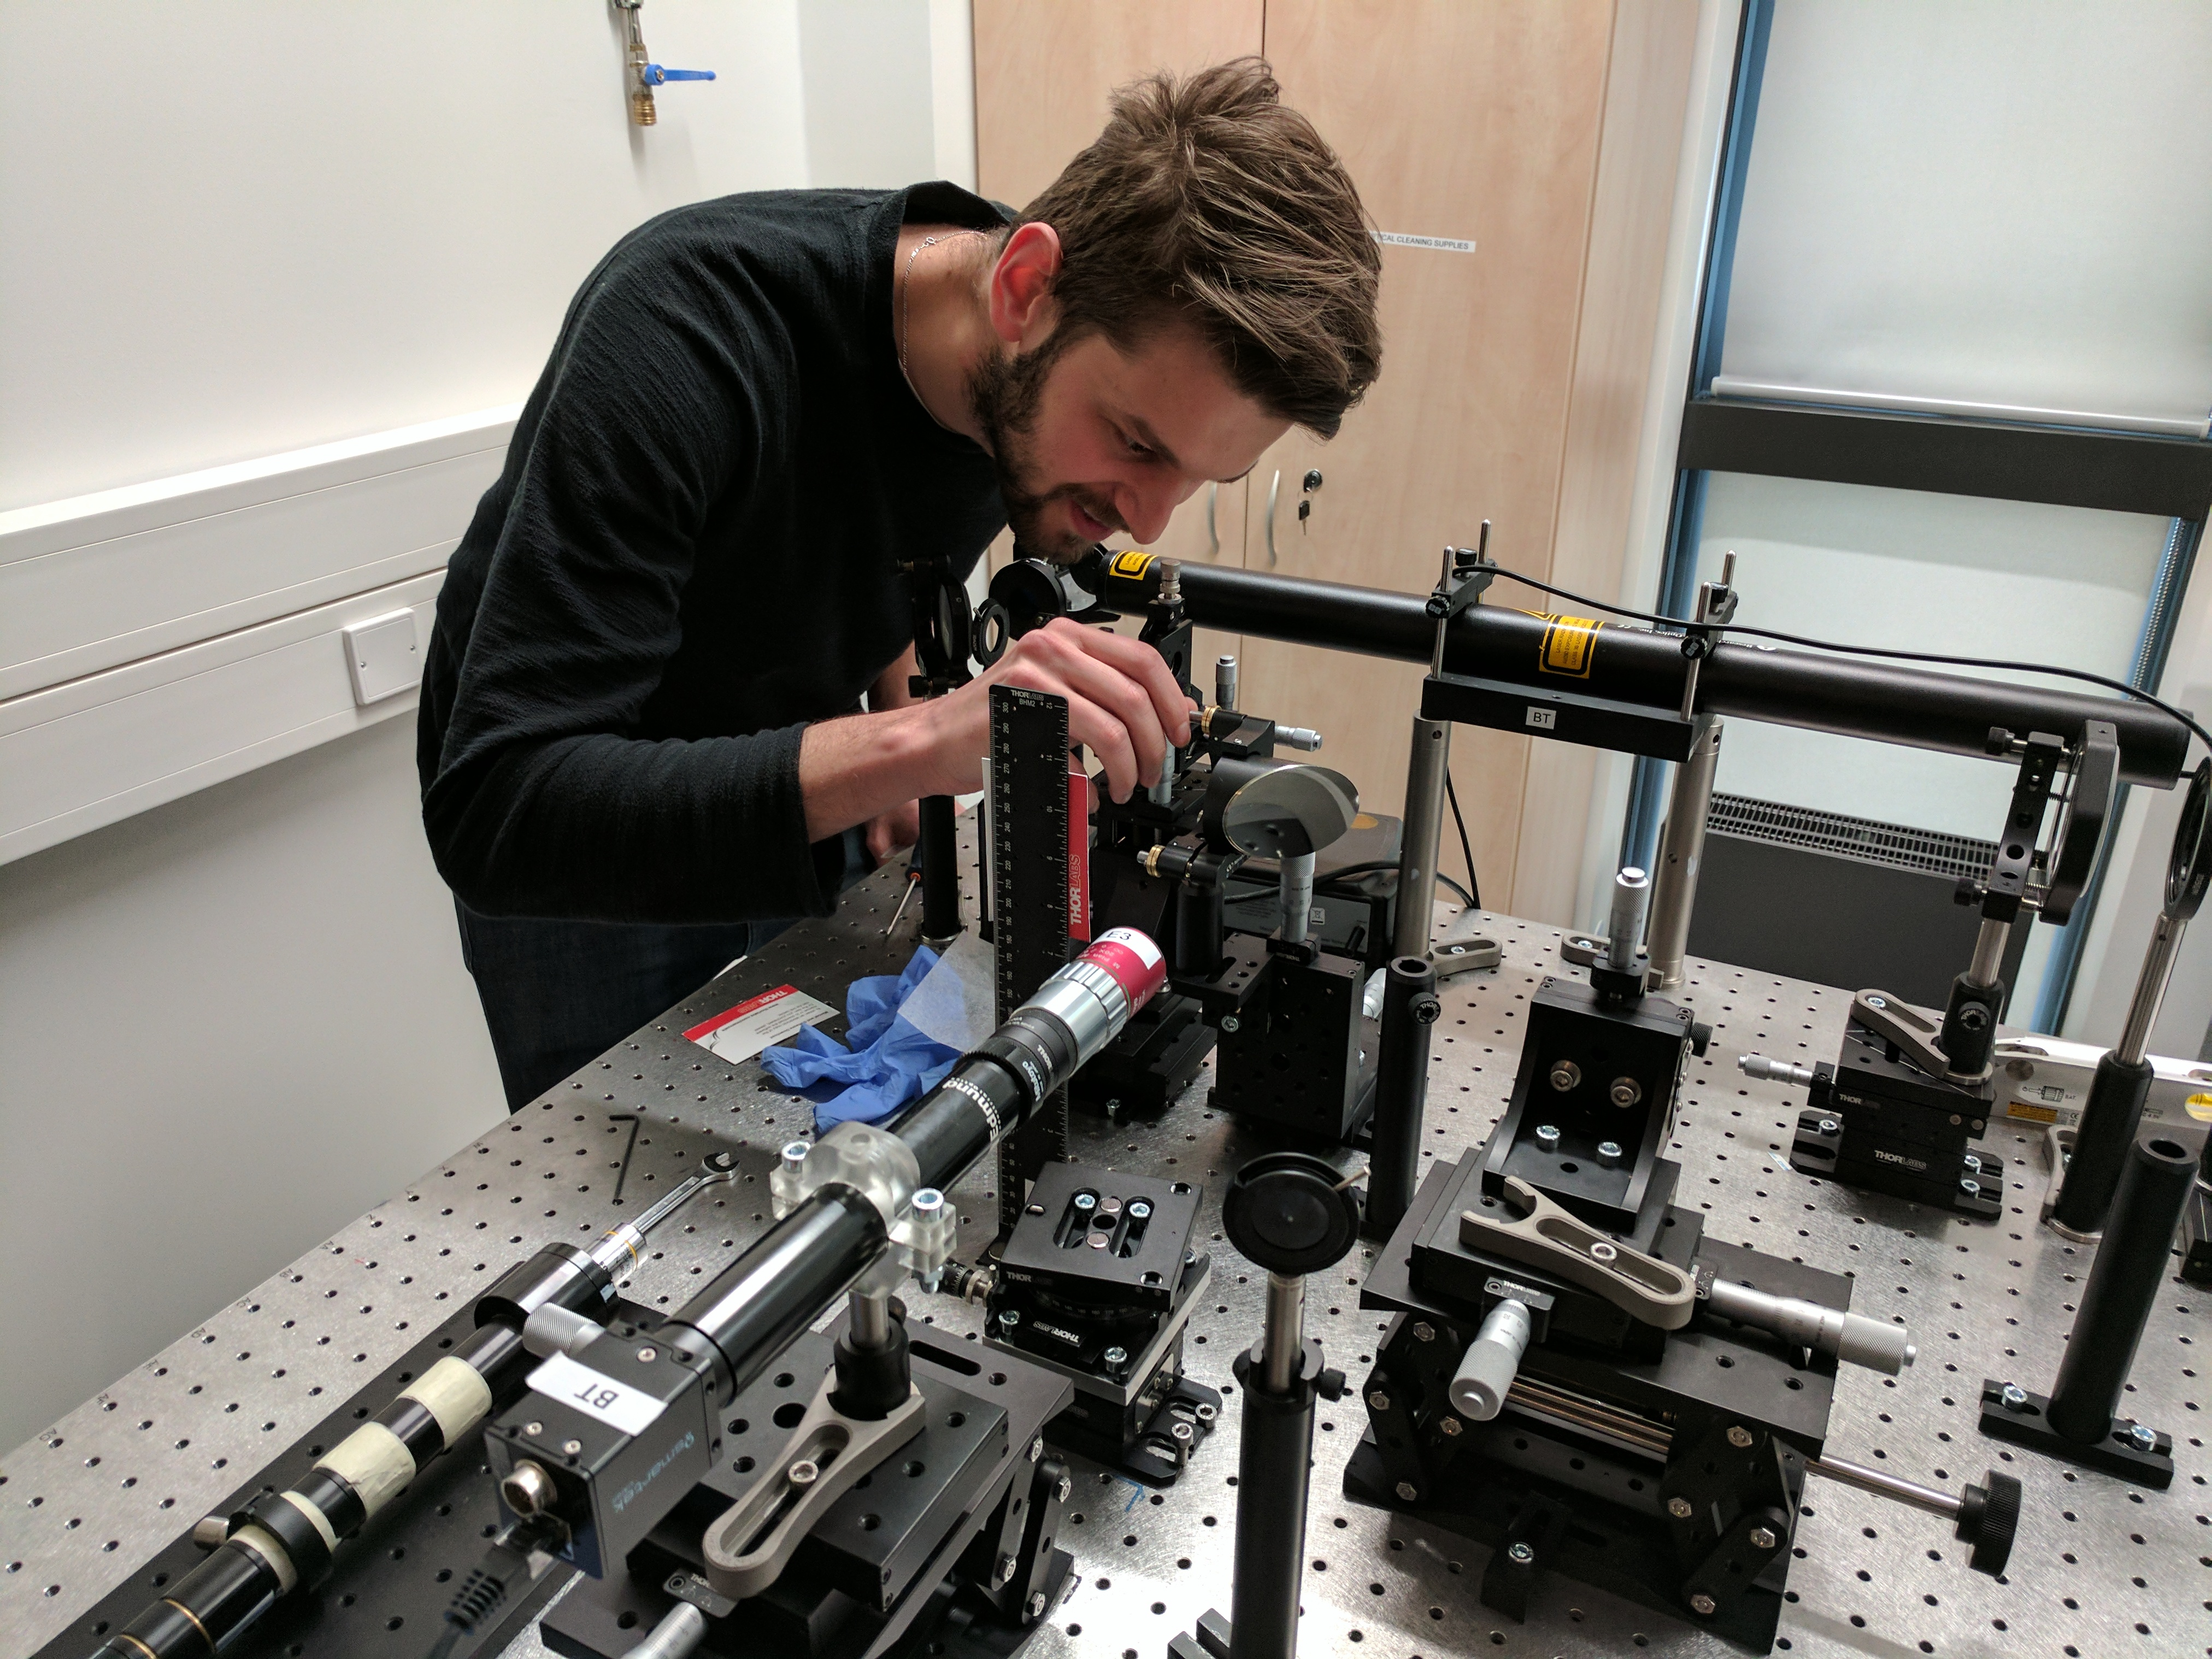
\includegraphics[width=0.4\linewidth]{./img/exp/photo.jpg}}}
	\caption{\textbf{(a)} Schematic diagram showing the experimental set-up for tight-focusing. The incoming laser beam is focused by a conventional off-axis parabolic mirror to the first focal point of the ellipsoidal plasma mirror. Beyond the first focus light diverges and is reflected from the dense plasma created on the surface of plasma mirror. The beam is then imaged to the second focal spot where the target should be placed. \textbf{(b)} Photo taken at Extreme Light Infrastructure (ELI) laser facility capturing a very long and frustrating procedure of the off-axis parabolic mirror set-up.}
	\label{fig:9}
\end{figure}

The diagram in fig. \ref{fig:9} - a schematically shows an experimental configuration for tight-focusing. A conventional off-axis parabolic mirror is aligned in such a way that the focus coincides with the first focal point of the ellipsoidal focusing plasma mirror. The ellipsoidal shape of the mirror provides point-to-point imaging, possesses no spherical aberration and allows relatively simple alignment procedure. The light reflected from the plasma mirror is then imaged to the second focal spot, where the target is placed. The fig. \ref{fig:9} - b shows the set-up of the off-axis parabolic mirror with an ellipsoidal plasma mirror in practice.